\documentclass[11pt]{article}
% ---------------------------------------------------------------------------
%  ccint project wrap-up — preamble
%  Compiles with pdfLaTeX (Overleaf default; no configuration needed).
% ---------------------------------------------------------------------------
\usepackage[T1]{fontenc}
\usepackage[utf8]{inputenc}
\usepackage{lmodern}
\usepackage[letterpaper,margin=1in,headheight=14pt]{geometry}
\usepackage{microtype}
\setlength{\emergencystretch}{3em}   % 允许必要时额外伸缩，消除长代码标识符造成的溢出

\usepackage{booktabs}
\usepackage{tabularx}
\usepackage{longtable}
\usepackage{array}
\usepackage{multirow}
\usepackage{amssymb}
\usepackage{amsmath}
\usepackage{enumitem}
\usepackage{fancyhdr}
\usepackage{titlesec}
\usepackage{graphicx}
\graphicspath{{figures/}}
\usepackage{tikz}
\usetikzlibrary{arrows.meta,positioning,calc,fit,backgrounds}
\usepackage[skins,breakable]{tcolorbox}

\usepackage[dvipsnames]{xcolor}
\definecolor{ink}{HTML}{1A1A1A}
\definecolor{accent}{HTML}{1F4E79}
\definecolor{warn}{HTML}{9C4221}
\definecolor{good}{HTML}{22543D}
\definecolor{rule}{HTML}{C8CDD4}
\definecolor{softbg}{HTML}{F4F6F8}
\definecolor{accentbg}{HTML}{EAF0F6}

\usepackage[font=small,labelfont={bf,color=accent},skip=8pt]{caption}

\usepackage[colorlinks=true,linkcolor=accent,urlcolor=accent,citecolor=accent]{hyperref}

% --- headers ---------------------------------------------------------------
\pagestyle{fancy}
\fancyhf{}
\renewcommand{\headrulewidth}{0.4pt}
\fancyhead[L]{\footnotesize\textcolor{accent}{ccint — Canada Cyber Social Intelligence}}
\fancyhead[R]{\footnotesize\thepage}

% --- section styling -------------------------------------------------------
\titleformat{\section}{\Large\bfseries\color{accent}}{\thesection}{0.7em}{}
\titleformat{\subsection}{\large\bfseries\color{ink}}{\thesubsection}{0.6em}{}
\titleformat{\subsubsection}{\normalsize\bfseries\itshape\color{ink}}{}{0em}{}
\titlespacing*{\section}{0pt}{2.2ex plus 1ex minus .2ex}{1.2ex plus .2ex}

% --- table helpers ---------------------------------------------------------
\renewcommand{\arraystretch}{1.18}
\newcolumntype{R}{>{\raggedleft\arraybackslash}X}
\newcolumntype{L}{>{\raggedright\arraybackslash}X}
\newcommand{\hd}[1]{\textbf{#1}}

% --- callout boxes ---------------------------------------------------------
\newtcolorbox{keybox}[1][]{
  enhanced, breakable, colback=accentbg, colframe=accent,
  boxrule=0pt, leftrule=3pt, arc=1pt, left=8pt, right=8pt, top=6pt, bottom=6pt,
  #1}
\newtcolorbox{warnbox}[1][]{
  enhanced, breakable, colback=softbg, colframe=warn,
  boxrule=0pt, leftrule=3pt, arc=1pt, left=8pt, right=8pt, top=6pt, bottom=6pt,
  #1}
\newtcolorbox{plainbox}[1][]{
  enhanced, breakable, colback=softbg, colframe=rule,
  boxrule=0.4pt, arc=1pt, left=8pt, right=8pt, top=6pt, bottom=6pt,
  #1}

% --- inline semantics ------------------------------------------------------
\newcommand{\code}[1]{\texttt{\small #1}}
\newcommand{\yes}{\textcolor{good}{\checkmark}}
\newcommand{\no}{\textcolor{warn}{$\times$}}
\newcommand{\noise}{\textcolor{warn}{noise}}

% --- verbatim-ish code block ----------------------------------------------
\usepackage{fancyvrb}
\DefineVerbatimEnvironment{shell}{Verbatim}
  {fontsize=\small,frame=single,rulecolor=\color{rule},framesep=6pt,
   formatcom=\color{ink}}

\geometry{margin=0.92in}
\setlist{topsep=3pt,itemsep=2pt,parsep=0pt}
\renewcommand{\arraystretch}{1.05}
\renewcommand{\topfraction}{0.92}
\renewcommand{\bottomfraction}{0.7}
\renewcommand{\textfraction}{0.06}
\renewcommand{\floatpagefraction}{0.85}

\title{\vspace{-1.7cm}\textbf{\color{accent}ccint --- Progress Brief}\\[3pt]
\large\color{ink} Canada Cyber Social Intelligence: design rationale, build, and
where it stands}
\author{}
\date{\normalsize 23 September 2026}

\begin{document}
\maketitle
\vspace{-1.5cm}

\section*{\color{accent}The question, and what changed about it}
\addcontentsline{toc}{section}{The question}

The project began as a longitudinal study: \emph{how does Canada-related
cybersecurity discussion change over time on social media?} A collector runs
continuously against Bluesky, posts are labelled under versioned schemes, and
change is tested statistically.

The first full analysis returned a negative result, and returned it with
enough rigour to be worth something. The largest topic movement in the 30-day
window, \code{data\_breach} at $+22\%$, has $p_{\mathrm{FWER}} = 0.734$ under
an author-level circular-shift null that preserves each author's volume, topic
mix and burstiness while destroying calendar alignment. Empirical power
analysis --- measured by author-pool replication rather than assumed ---
puts the requirement at roughly $8\times$ the current volume.

That result is only interesting if one knows what produced it. Three
explanations were open, and nothing in the system could separate them, because
every figure it produced came from labels it had produced itself. The work of
the last phase was to build the measurements that can separate them. They do,
and the answer was not the expected one: \textbf{the shortfall is not in the
statistics and not mainly in the labelling --- it is that the platform carries
almost no human discussion of these events at all.}

\section*{\color{accent}Why the system is built this way}

Four commitments shaped every design decision. Each exists to prevent a
specific failure that would be invisible after the fact.

\paragraph{Bluesky, and one platform only.}
An open, documented API with usable historical search and terms that permit
research collection; X and Reddit were excluded on access grounds rather than
merit. The consequence is stated rather than hidden: this is a convenience
sample, and the project's job became partly to measure what it can show.

\paragraph{Labels are versioned and never overwritten.}
Annotation rows are keyed by (post, annotator version) and only ever inserted;
four schemes coexist over the same corpus and diff row by row. Without this,
every improvement to the annotator would silently rewrite history, and a shift
in topic distribution could never be attributed to the world rather than to the
method.

\paragraph{Raw data is kept verbatim; every number carries provenance.}
Payloads are stored unmodified, and every run and model label records what
produced it, including the SHA-256 of the exact prompt text. That last part was
added after noticing that a model annotator's output is entirely determined by
its prompt: ``labels are never overwritten'' had preserved the labels while
losing the conditions that made them.

\paragraph{System failure must be distinguishable from social change.}
Every collection path records mode, status, window and counts, so a day with
half the usual volume is attributable to either the world or a token expiry. The
principle held under test: a 42-run token outage appears as 42 \code{partial}
runs, not as a drop in Canadian cyber discussion.

\begin{keybox}
Underlying all four: \textbf{measure before improving.} Repeatedly the
intuitive next step turned out to be aimed at the wrong quantity, and only
measurement revealed it --- tuning the trend score would have been wasted,
relaxing the relevance rules helps but not for the population that seemed to
need it, and the most recent prompt improvement introduced a regression the
evaluation set certified as correct.
\end{keybox}

\begin{figure}[htbp]\centering
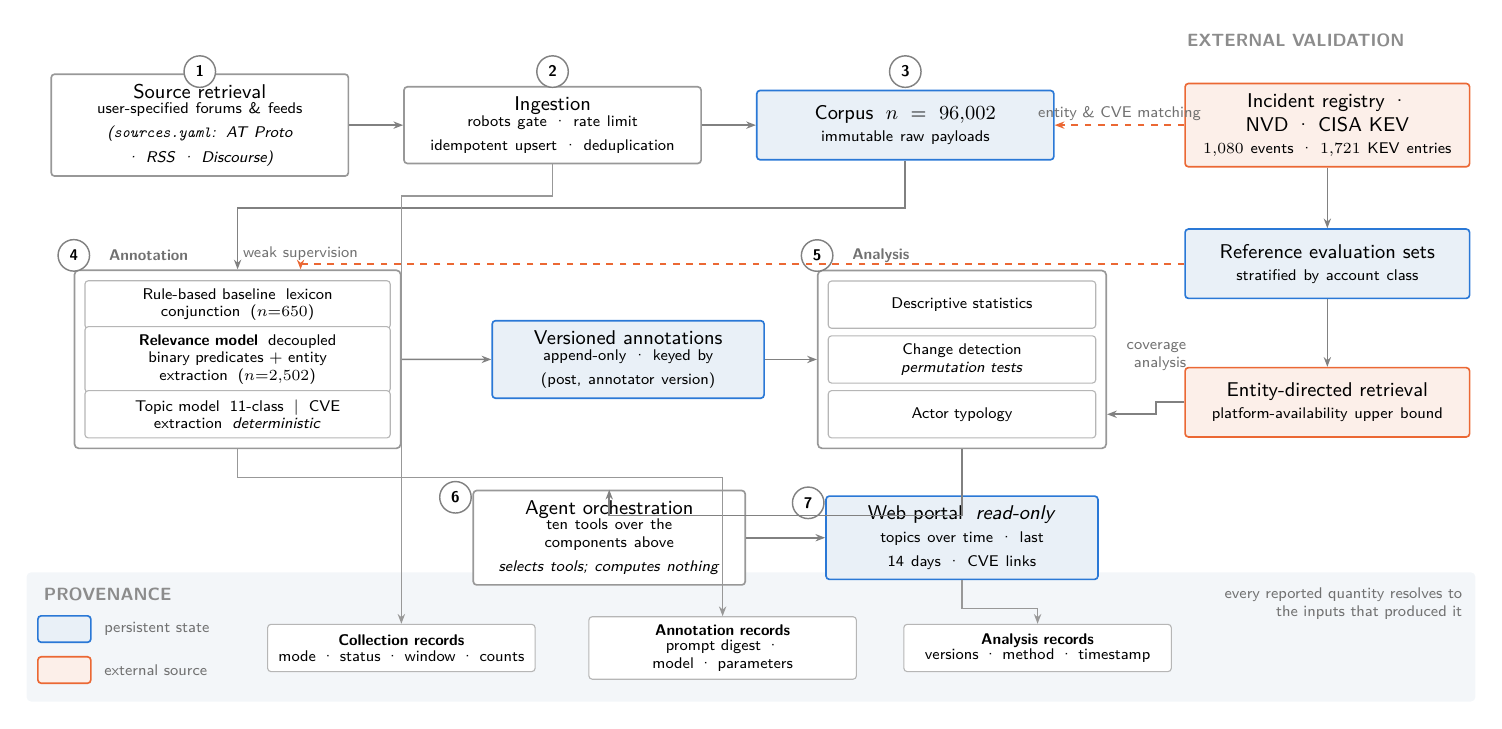
\includegraphics[width=0.86\linewidth]{Architecture.png}
\caption{Processing pipeline. Stages 1--3 acquire and store the corpus, stage 4
annotates it under coexisting versioned schemes, stage 5 analyses the result.
The external-validation column supplies labels no component of the pipeline
produced.}
\label{fig:arch}
\end{figure}

\section*{\color{accent}How it was built}

Collection runs in two modes against the fixed term list --- a day-by-day
backfill and an hourly incremental --- with idempotent ingestion, stale-run
reaping and client-timestamp repair; the corpus stands at 95{,}943 posts across
three sources. Annotation proceeded in four generations,
all retained: two lexicon-based, one that re-decides topic only while
inheriting the relevance verdict verbatim so the two changes stay separately
attributable, and one that replaces the relevance decision entirely. Analysis
covers descriptive statistics, permutation testing against two null models,
behavioural broadcast detection with a collection-lag control, and a two-axis
actor typology separating measured audience from content-judged function. The
most recent phases added the external-validation column of
Figure~\ref{fig:arch} and then three capability layers: user-specified sources,
deterministic CVE linking, and a read-only portal.

\paragraph{Sources are configuration, not code.}
\code{config/sources.yaml} names the forums and feeds to read; two generic
collectors (RSS\slash Atom and the Discourse public JSON API) cover most of what
a security community exposes. Both consult \code{robots.txt} and refuse a source
they cannot read, because a collector that gets blocked produces a gap, and a
gap is indistinguishable from a fall in discussion --- the confusion this project
exists to prevent. Each source must declare why automated access is believed
permissible; the loader rejects one that does not. Web sources reuse the
existing ingest path rather than adding a second, since a second path is a
second way to bypass run bookkeeping.

\section*{\color{accent}Where it stands}

\subsection*{The collection boundary was never measured}

The 34 search terms came from a specification naming four examples followed by
``etc.''; the remaining 26 were supplied during implementation from domain
intuition, never derived from data and never revised. Reconstructing per-term
productivity offline over the stored corpus:

Productivity is close to degenerate. \code{cybersecurity} returned 22{,}498
posts and 200 relevant ones; \code{ransomware} 8{,}881 and 105; \code{CVE}
12{,}502 and \textbf{three}. Eleven terms returned no relevant post at all, and
one returned no post at all. \code{CVE} accounts for $13.7\%$ of everything
collected; \code{cybersecurity} alone accounts for $30.8\%$ of all relevant
posts, so the corpus time series is, to first order, one search term's
time series, and nothing monitors it. None of the 34 terms names Canada, so
any Canadian cyber post not phrased with one of them is unreachable by
construction.

\subsection*{Replacing the relevance gate}

The old decision was a conjunction of two narrow lexicons, so recall was
bounded by their intersection: 650 of 91{,}551 posts passed and the 89{,}714
rejected had never been examined by anything semantic. The replacement poses
two \emph{independent} predicates rather than one conjunction --- a single
combined prompt causes a 4B model to collapse the conjunction onto the side it
knows better, admitting global threat-intelligence noise at $6.8\%$ against a
true Canadian rate of $1.1\%$.

\begin{center}\small
\begin{tabularx}{.93\linewidth}{@{}Lrrr@{}}
\toprule
\hd{Relevance gate} & \hd{recall} & \hd{specificity} & \hd{corpus} \\
 & \hd{@ registry} & \hd{@ registry} & \hd{relevant} \\
\midrule
\code{rules\_v2} --- keyword conjunction     & 46.5\% & 99.8\% & 650 \\
\code{llm\_v2c} --- two questions + validation & \textbf{68.3\%} & 99.4\% & \textbf{2{,}348} \\
\bottomrule
\end{tabularx}
\end{center}

Of the 1{,}799 posts newly admitted, $84.0\%$ had been rejected on the Canadian
side of the conjunction. Two results here are method rather than number. Entity
offsets are computed with \code{str.find} rather than requested from the model,
on the narrow grounds that small models miscount them --- which turned into a
free hallucination detector, since an entity that cannot be located in the post
was invented, and nearly half of extracted \code{place} entities failed it. And
the residual error is neither a prompt nor a capability problem: the posts still
missed carry no country marker at all, so closing it needs a gazetteer of
Canadian organisations, not a larger model.

\subsection*{The external reference, and the central result}

Until this phase every precision and recall figure traced to a single author
who wrote the rules, the prompts, and the hand-coded evaluation set. A
reported $\kappa = 0.870$ measured agreement under those conditions, not
independence. Ingesting a public ransomware victim registry (1{,}080 events,
1{,}943 entities) supplies labels no part of the system produced.

For every Canadian event in the window, the victim organisation's name was
also searched directly on the platform, with no cybersecurity term attached,
and every hit passed through the cyber judgement before counting:

\begin{center}\small
\begin{tabularx}{.93\linewidth}{@{}Lrr@{}}
\toprule
\hd{Canadian ransomware events, 22 Aug -- 22 Sep 2026} & \hd{Events} & \hd{Share} \\
\midrule
Listed in the registry                                   & 27 & --- \\
At least one cyber-related post exists on Bluesky        & 26 & 96\% \\
At least one such post was collected by ccint            & 26 & 96\% \\
At least one came from a \textbf{non-feed} account       & \textbf{2} & \textbf{7\%} \\
\bottomrule
\end{tabularx}
\end{center}

The 144 relevant posts come from 15 accounts. Twelve are automated
threat-intelligence feeds; the three that are not are Canadian news
organisations contributing five posts between them, all about a single event.
Individual users contributed nothing; $94.9\%$ of the posts have no likes.

\begin{keybox}
\textbf{What looks like coverage is syndication.} The collector is not the
bottleneck here --- it captured 26 of the 26 events the platform carried. No
ransomware trend is detectable because there is almost no ransomware
\emph{discussion} to detect: the corpus is a near-complete mirror of several
leak-site feeds. That also reframes the power analysis --- $8\times$ of this
corpus is $8\times$ as much syndication, so volume is the wrong lever.
\end{keybox}

The one exception is instructive. The Commission de la construction du
Qu\'ebec, listed by the Qilin group with roughly 350{,}000 records taken, drew
genuine Canadian media coverage in both languages. Four of the five posts are
in the corpus; the fifth, a radio interview with the CCQ's chief executive,
carries no term from the 34-term list because \emph{protection pr\'eventive} is
in no lexicon --- the collection-boundary gap at human scale.

\subsection*{Linking discussion to vulnerabilities}

CVE identifiers are extracted by regular expression, not by a model. The format
is fixed by MITRE, so the extraction is deterministic --- which makes this the
one table in the system whose trustworthiness does not depend on annotation
quality. Identifiers are then enriched from two independent external sources:
NVD supplies theoretical severity, and the CISA Known Exploited Vulnerabilities
catalogue records that exploitation has actually been observed. The two are kept
in separate columns and deliberately never combined into a single risk score:
one is a judgement about how bad a flaw could be, the other is an observation
that someone is using it, and merging them would conceal which part is external
fact.

Across the corpus, 10{,}820 posts mention 5{,}404 distinct CVE identifiers.
Only 147 of those --- $2.7\%$ --- appear in the KEV catalogue. Those 147 attract
$19.3\%$ of all mentions, a concentration of roughly $7\times$, and 22 of the 25
most-discussed identifiers are among them.

\begin{keybox}
\textbf{Attention tracks exploitation, not severity.} This is the first result
in the project where social-media attention aligns with an external ground truth
rather than merely mirroring a feed. It is also a usable one: a monitor that
ranks vulnerabilities by how much they are being discussed recovers, without
being told, most of the set that CISA has independently confirmed as exploited.
\end{keybox}

\subsection*{A methodological result about evaluation}

The prompt revision that fixed entity recall simultaneously generalised ``a
\code{.ca} domain counts'' into ``a domain counts'', inflating the corpus from
906 to 3{,}528 posts with a third of them spurious --- while the external
negative set reported $99.0\%$ specificity throughout, because it is built from
formulaic English feed posts about foreign victims and contains none of the
model's actual failure modes. \textbf{An external label removes self-reference
but does not confer representativeness, and a non-representative evaluation set
does not merely fail to catch a regression --- it certifies one.} Two
deterministic checks catch it at no cost; the accompanying iteration report
gives the full account.

\section*{\color{accent}What the project is, and what comes next}

The original framing --- trend analysis of Canadian cyber discourse --- is not
available at this volume for this event class, and adding data will not make it
so. What is available, and appears to be unreported in the surveyed
literature, is a sensor that states its own blind spots numerically. Published
systems report how many events they detected (84 of 151 in the strongest
comparable work); none reports how many events had no platform presence at
all, because establishing that requires the per-event entity-directed
retrieval used here, affordable only when the event count is small. This project's greatest
liability --- a corpus of a few thousand relevant posts --- is precisely what
makes the denominator measurable.

Immediate priorities, in order:

\begin{enumerate}[leftmargin=1.5em,itemsep=2pt]
\item \textbf{Widen the registry beyond ransomware} --- advisories, KEV,
Canadian media. Every figure above is conditioned on a source that sees only
leak-site victims: the narrowest limitation in the work.
\item \textbf{Feed the registry back into the relevance decision.} The residual
failure is missing knowledge of Canadian organisation names, and the registry
is a list of exactly those names.
\item \textbf{Add a Canada-side query stream} as an additional disjunctive
stream, not a filter, to reach the population the registry cannot see.
\item \textbf{Have an independent annotator label the 200-post sample} already
drawn and left blank --- the one step that cannot be automated.
\item \textbf{Let the new sources accumulate.} Multi-source collection works but
is not yet demonstrated at scale: the two feeds added so far contributed 45
posts, because RSS exposes only recent items and cannot be backfilled. A
comparable time series requires either running them forward for weeks or adding
a paginated source such as a Discourse forum.
\end{enumerate}

\medskip
\noindent{\footnotesize\itshape\color{ink!65}
Corpus 95{,}943 posts across three sources, 22 Aug -- 23 Sep 2026; registry and
KEV catalogue retrieved 22--23 Sep 2026; five coexisting annotation versions;
252 tests passing. Methodology in the
project wrap-up, coverage measurements in the iteration report.}

\end{document}
